\section{Vandfalds-Modellen}\label{sec:vandfald}
Vandfalds-modellen er en sekventiel procesmodel som består 
af 5-7 forskellige faser. Hver fase er en essentiel del af udviklingen
og bygger ovenpå den forgående fase, og er et krav for at starte næste.\\

Anvendes en Vandfaldsmodel til et software projekt, laves en kontrakt med
kunden, som indeholder krav, specifikationer og funktionalitet til at 
dække hele systemet. Prisen bliver fastlagt samt en tidsplan for forventet
levering af systemet. Efter underskrift designes systemet og hvert trin i 
modellen følges indtil det endelige produkt, baseret på de fastlagte krav,
er klar til levering.\\

En af ulemperne ved et stort projekt, som følger vandfaldsmodellen er, 
at der kan gå måneder, hvis ikke halve år før kunden ser produktet første gang.
Krav, specifikationer og funktionaliteter kan forstås på mange måder, hvilket
medfører en risici. Har kunden ikke været god til at udtrykke og beskrive 
produktet, kan det forventede og det faktuelle produkt være langt fra 
hinanden.\\

Er produktet omfattende og kompliceret, kan ændringer heraf tage
lang tid og kræve mange resourcer. Især hvis ændringerne findes i enten 
arkitekturen eller selve funktionaliteten af systemet. 
Kunden skal selv betale for disse ændringer udover den aftalte fastlagte 
pris, samt være indforstået med at skuppe tidsplanen tilsvarende.\\
  
Vandfalds-modellen kan ses på Figur \ref{fig:waterfallmodel} \\


\begin{figure}[H]
    \centering
    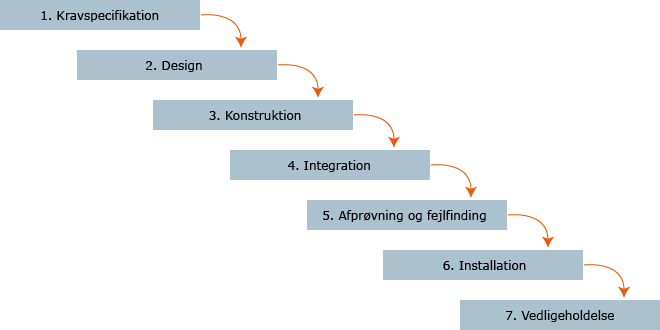
\includegraphics[width=0.7\textwidth]{figures/waterfall.png}
    \caption{Vandfaldsmodellen \cite{WaterfallModel}}
    \label{fig:waterfallmodel}
\end{figure}

I forbindelse med mindre projekter, hvor produktet er nemt at
definere, ændringer ikke forventes at forekomme og perioden minimal, 
anvendes vandfaldsmodellen med fordel.


\section{Agile metoder}\label{sec:agilemetoder}
Agil er en betegnelse for en række iterative softwareudviklingsmetoder, hvor der løbende leveres små dele af 
produktet til kunden. Agile udviklingsmetoder er oftest kendetegnet ved Det Agile Manifest \cite{AgileManifesto}.
Manifestet beskriver blandt andet hvordan samtaler og møder med kunden, samt god, fungerende software er i fokus, 
fremfor en lang liste af processer og værktøjer og fuldstændig dokumentation. \\

Ved udvikling af større softwaresystemer, hvor kunden er en nær kontakt igennem udviklingsperioden, kan udviklerteamet
drage stor fordel af at udvikle agilt. Dette skyldes at agile metoder bygger på \textit{continual improvement},
hvilket vil sige at produktet bliver udviklet inkrementelt, sådan at man altid har noget at vise kunden. Desuden er en fordel ved agile
metoder at de er omstillingsparate. Dette skyldes at man kun planlægger sit arbejde få uger frem.